\chapter{Synthèse}
\label{sec:synthese}
\section{Les résultats et améliorations possibles}

Mon stage a été l'occasion de réaliser de nombreuses missions. Ces dernières étaient plus ou moins importantes mais toutes ont été l'occasion d'apprendre de nouvelles choses et de mieux comprendre comment fonctionne l'application. Les missions les plus importantes restent le didacticiel ainsi que la remise en place de l'affiliation. En effet le nouveau système d'affiliation est aujourd'hui en place dans tous les restaurants qui possèdent cette option. Le premier restaurant que j'ai brièvement énoncé lorsque je parlais des 50 tablettes a été le premier à mettre ce nouveau système d'affiliation en place et jusqu'à ce jour nous n'avons pas connu de problème. 

L'autre mission importante du stage est le tutoriel. C'est la mission qui m'a demandé le plus de temps car il a fallu tout inventer, que ce soit la structure, le côté graphique avec le XML, la logique entre les étapes etc. C'est aussi pour cela que cette mission à été très intéressante. Cependant ce qui a été développé jusque-là n'est qu'une première version. Par conséquent il est fort possible que le tutoriel soit amélioré. D'ailleurs, à ce stade de développement on peut déjà penser à des améliorations côté visuel comme côté code. Celle qui me vient le plus à l'esprit concerne l'éclaircissement des éléments. Techniquement on utilise des coordonnées en "dur" pour les rectangles éclaircis. C'est d'ailleurs quelque chose qui a pris du temps de développement. J'ai du étalonner en faisant plusieurs essais avec différentes valeurs. Pour certaines vues les coordonnées sont récupérées. Pour d'autre les vues sont dans d'autres layouts et il est plus difficile de les obtenir car ce ne sont pas des vues d'Android mais de l'application propre et les récupérer enclenchait des bugs. C'est d'ailleurs pour cela qu'il y a des redéfinitions de fonctions dans les fonctions de type "setBrightView". Il y a des cas où l'on a un seul paramètre et c'est la vue et d'autre ou on a les coordonnées. Une autre amélioration possible est de donner plus de "pouvoir" à l'utilisateur (ici comprendre le restaurateur). Il pourrait par exemple dans le futur avoir la possibilité de gérer lui-même ses étapes de tutoriel, choisir ses couleurs de pop-up etc. Il a aujourd'hui seulement la possibilité de changer les textes.

Pour toutes les missions énoncées, ces dernières ont été mises en production et le résultat est qu'aujourd'hui l'utilisateur à accès à ces nouvelles fonctionnalités. Comme expliqué précédemment certaines sont optionnelles (affiliation, didacticiel). L'avantage pour les clients est que les nouvelles fonctionnalités sont intégrées à l'offre Tastycloud. Par conséquent ce sont des sortes de promesses que fait l'entreprise et le client reçoit ces ajouts. Bien évidemment, ces fonctionnalités sont souvent en rapport avec des demandes clients ou du feedback mais d'autres clients pouvaient n'avoir rien demandé et c'est une réelle plus-value pour le client qui est alors témoin du sérieux et de l'efficacité de la solution.

\section{Ce que j'ai appris}

Ce travail chez Tastycloud m'a appris des notions de développement plus poussé que lors de mes précédents stages. J'ai, en effet ici appris à mettre en oeuvre un schéma d'utilisation et à conceptualiser et modéliser un système informatique. Cela a été très enrichissant et stimulant d'un point de vue ingénierie car on a le sentiment d'avoir avancé en compétence par rapport à ce qu'on a pu faire par le passé. D'un point de vue plus technique j'ai appris un nouveau langage kotlin et de nouveaux principes Android. J'ai appris des choses côté graphique avec le XML. C'est un stage qui demande beaucoup d'autonomie dans les recherches c'est aussi pourquoi j'ai appris à bien cibler mes recherches pour trouver des solutions efficaces rapidement. 

Comme c'était la première fois que j'étais confronté à un cas concret d'application Android j'ai aussi été sensibilisé au fonctionnement d'une application dans le monde de l'entreprise. Cela a été intéressant de voir comment marchait l'évolution de la maintenance de ce genre d'application. D'un point de vue moins technique j'ai aussi été confronté au travail en start-up et également en openspace qui est aussi une expérience formatrice.

    
\chapter{Conclusion}
\label{sec:conclusion}

En conclusion, ce stage chez Tastycloud à été une expérience enrichissante, formatrice, intéressante et même conviviale ! J’ai été amené tout au long du stage à faire preuve d’autonomie dans la recherche d’informations et également à découvrir un tout nouveau milieu : celui de la start-up. J'ai aussi été sensibilisé au monde de la restauration pour bien comprendre les spécificités de l'application. Chaque restaurant a ses propres caractéristiques et son propre vocabulaire, ses propres besoins auxquels il faut s'adapter. J'ai donc appris toutes ces choses au fur et à mesure et avec l’aide principalement de mon tuteur et au reste de l'équipe.

J'ai développé des compétences techniques que ce soit en Kotlin ou Android. Bien que j'ai été dans un premier temps un peu perdu surtout en commençant par la mission de l'affiliation. J'ai réussi à me former en apprenant par moi-même et avec l'aide de mon tuteur. Les sites web tels que "stackoverflow" m'ont aussi bien aidé pour comprendre certains détails techniques que ce soit encore une fois en Android ou en Kotlin. J'ai dorénavant bien conscience de la manière dont fonctionne l'application et tous les enjeux autours. Je pourrai, je pense, réutiliser toutes ses connaissances dans le futur surtout que je souhaite m'orienter dans le développement mobile. Enfin, ce stage a été un bon exemple de pourquoi il faut documenter son code, pourquoi il est important de poser des schémas et des diagrammes UML avant de commencer le développement d'un projet la réflexion étant mise en avant tout le long du projet. Cette réflexion se fait d'un point de vue utilisateur (comment va-t-il utiliser cette fonctionnalité ?) ou d'un point de vue réutilisation du code, ce qui a été énoncé durant le rapport.

Cette partie du stage s'est donc bien déroulée. Cependant ce dernier se termine en août et par conséquent j'ai de nouvelles missions qui m'attendent cet été. Notamment une mission de customisation des produits (par exemple choisir les ingrédients de sa pizza). Je suis ainsi fier de participer aux enjeux de l’entreprise à travers les missions qui m’ont été confiées. Le projet de Tastycloud étant innovant et original il m'a été facile de me motiver pour y travailler surtout qu'on m'a donné une certaine liberté dans le développement. Savoir que certaines des fonctionnalités que j'ai développées peuvent être utilisées par des milliers de clients est une immense satisfaction. C'est pour tout cela que Tastycloud est pour moi une expérience élémentaire de mon parcours universitaire.

\begin{figure}[!htp]
  \centering
  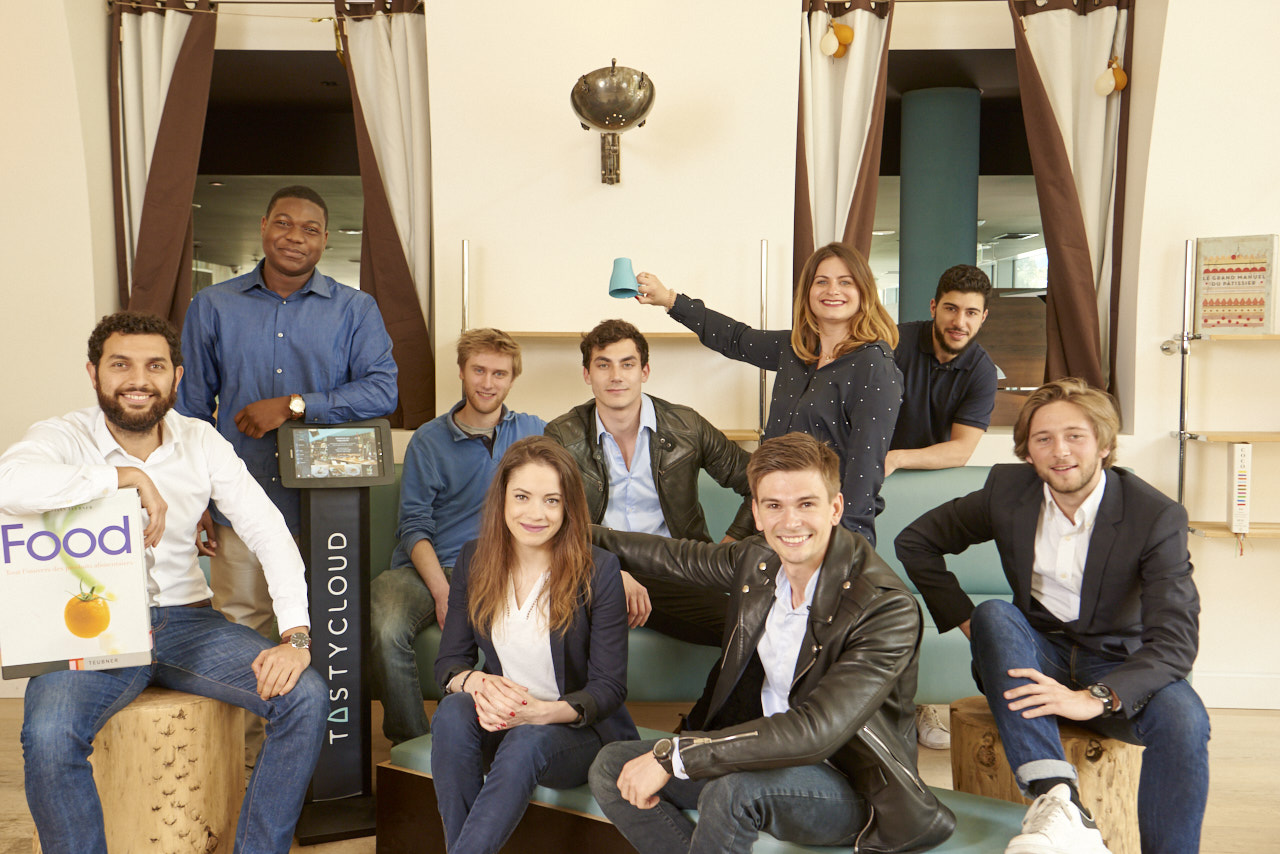
\includegraphics[width=130mm,scale=0.5]{images/equipe.jpg}
  \caption{Photo de l'équipe}
  \label{fig:boat1}
\end{figure}

\chapter{Annexe}
\label{sec:annexe}

\underline{Fonctionnement du système presenter, controller, adapter ... :}

\begin{figure}[!htp]
  \centering
  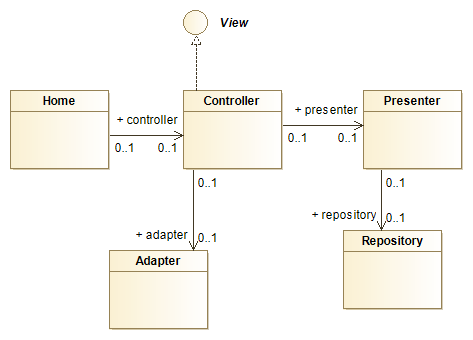
\includegraphics[width=130mm,scale=0.5]{images/diagramme_conttroller.png}
  \caption{Fonctionnement du système "controller"}
  \label{fig:boat1}
\end{figure}

Ce système marche avec Dagger. Repository est la classe qui fait lien avec la base de données et Home appelle les controller.

\underline{Texte du didacticiel :}

1) Bonjour et bienvenue chez X ! Nous allons vous montrer comment passer commande depuis cette tablette.
Cela ne vous prendra que quelques secondes.
Non, merci / Continuer

2) Retrouvez ici les suggestion de l'établissement.
Suite

3) Allergique ou intolérant ? Sélectionnez ici les éléments qui vous concernent, une icône apparaitra alors sur les produits qui en contiennent.
Suite

3) Naviguez entre les différentes catégories pour faire votre choix.
Suite

4) Cliquez sur un produit pour en voir tous les détails.
Suite

5) Vous désirez autre chose ? Appuyez sur la flèche pour revenir à l'écran précédent
Suite

6) Celui-ci vous plait et vous souhaitez le commandez ? Cliquez sur "mémoriser" ou sur "personnaliser et mémoriser" s'il y a des options à choisir pour l'ajouter à votre sélection.
Suite

7) Une fois votre choix fait, retrouvez les plats que vous avez retenus dans l'onglet "sélection".
Suite

8) Votre sélection vous convient et vous êtes prêts à commander ? Cliquez sur "envoyer ma commande en cuisine", un serveur viendra vous apporter votre premier plat dès que le chef l'aura préparé.
Suite

9) Si malgré tout vous avez des doutes, n'hésitez pas à appeler un serveur qui viendra vous aider avec grand plaisir. Bon appétit !
Fin

\clearpage
\underline{Capture d'écran didacticiel :}

\begin{figure}[!htb]
  \centering
  \begin{minipage}[b]{0.45\textwidth}
    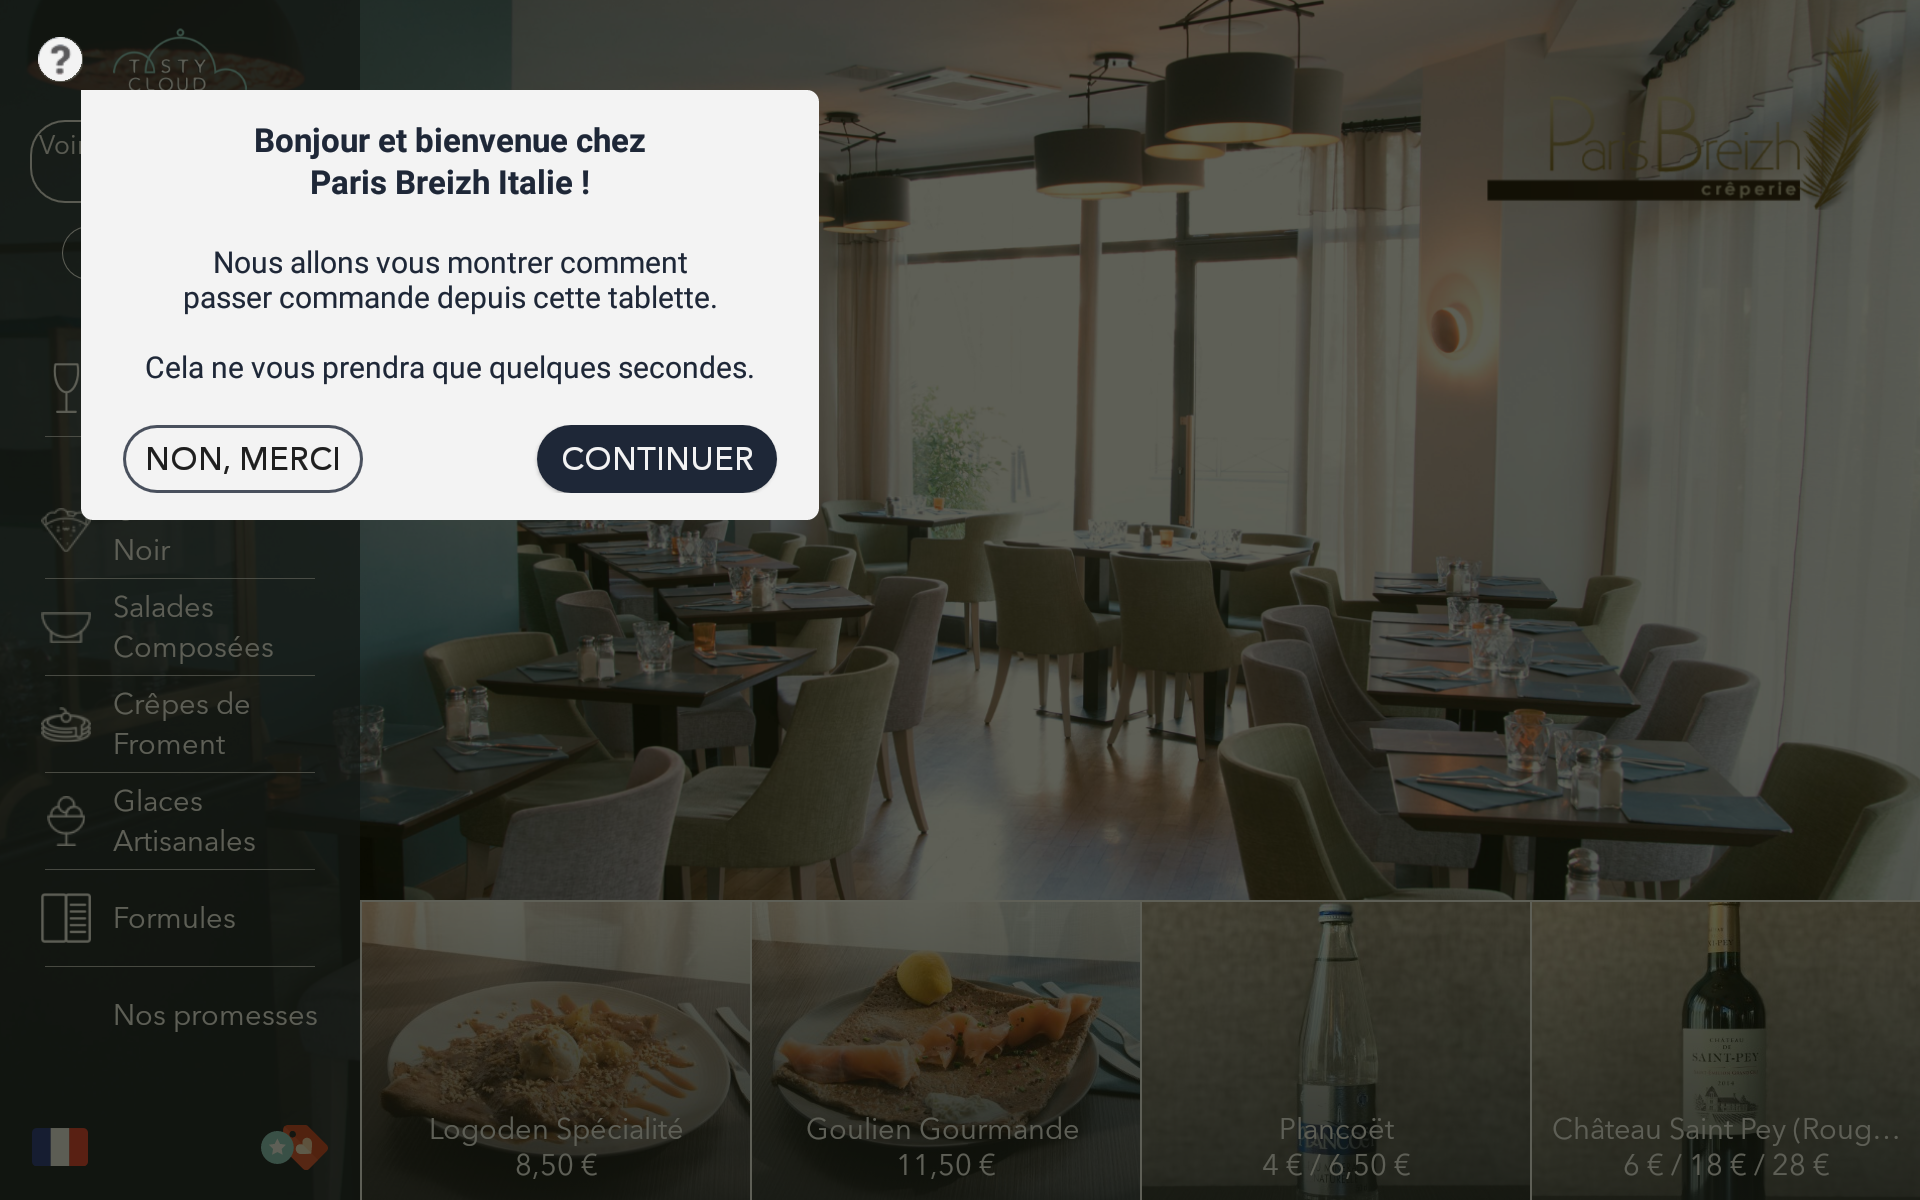
\includegraphics[width=\textwidth]{images/tuto7.png}
    \caption{Message bienvenue}
  \end{minipage}
  \hfill
  \begin{minipage}[b]{0.45\textwidth}
    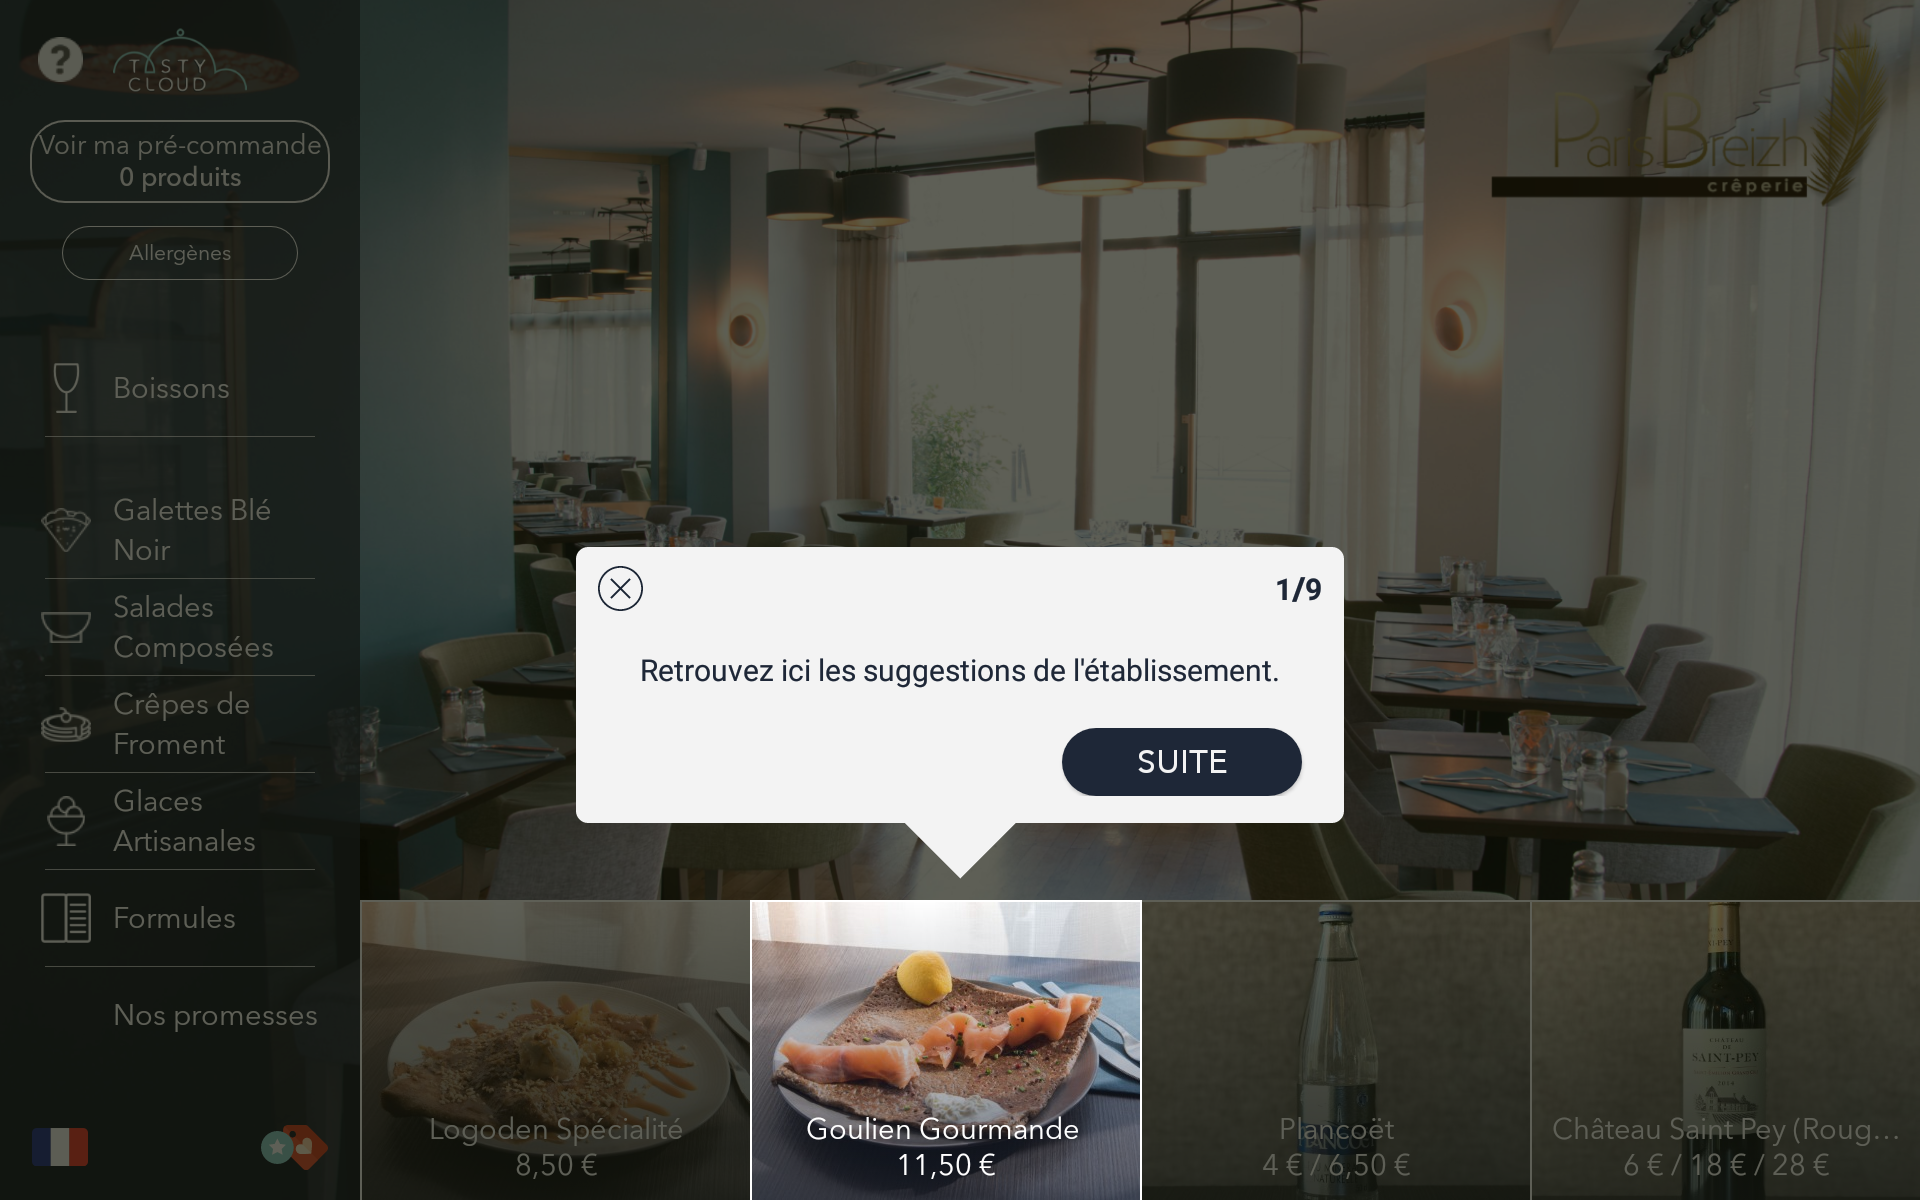
\includegraphics[width=\textwidth]{images/tuto2.png}
    \caption{Étape 1}
  \end{minipage}
\end{figure}

\begin{figure}[!htb]
  \centering
  \begin{minipage}[b]{0.45\textwidth}
    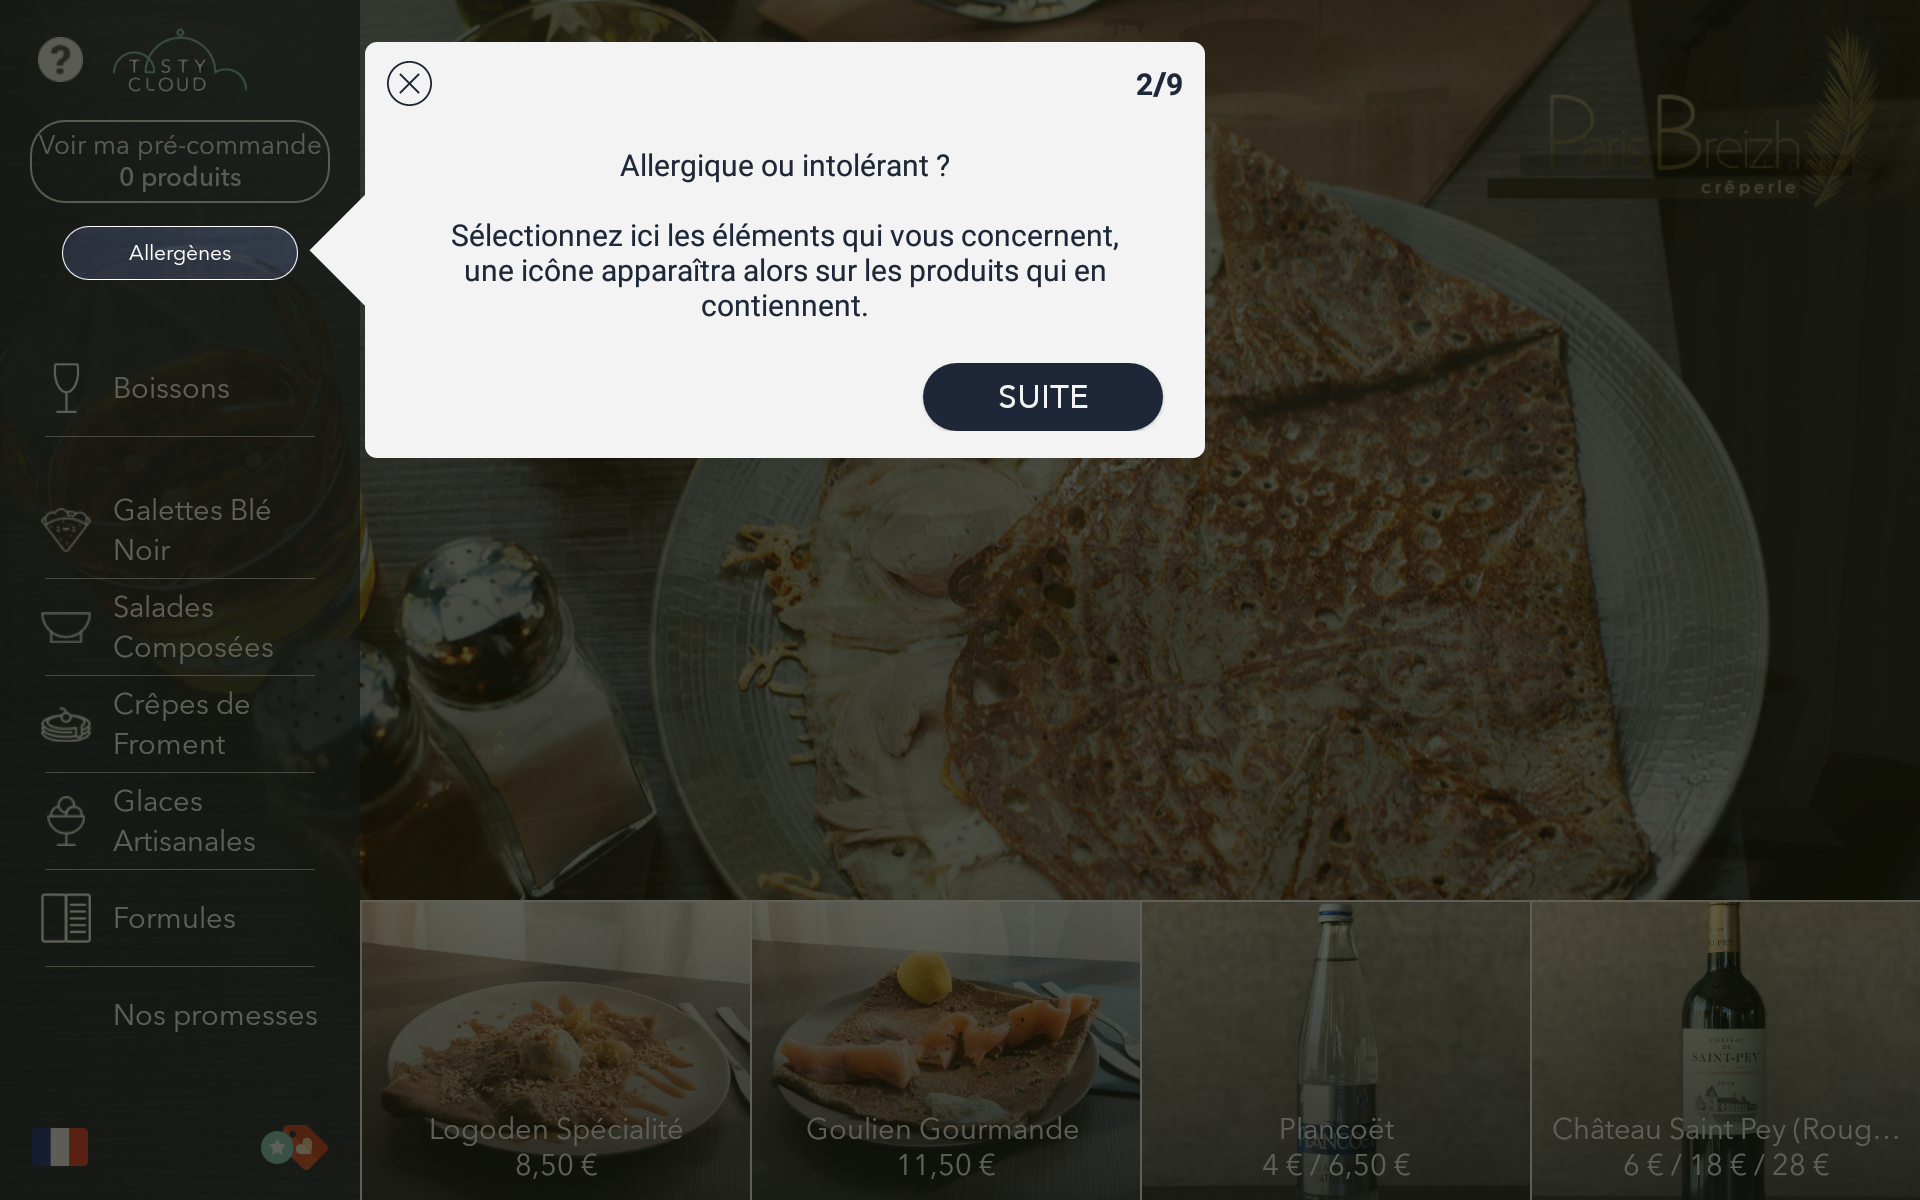
\includegraphics[width=\textwidth]{images/tuto3.png}
    \caption{Étape 2}
  \end{minipage}
  \hfill
  \begin{minipage}[b]{0.45\textwidth}
    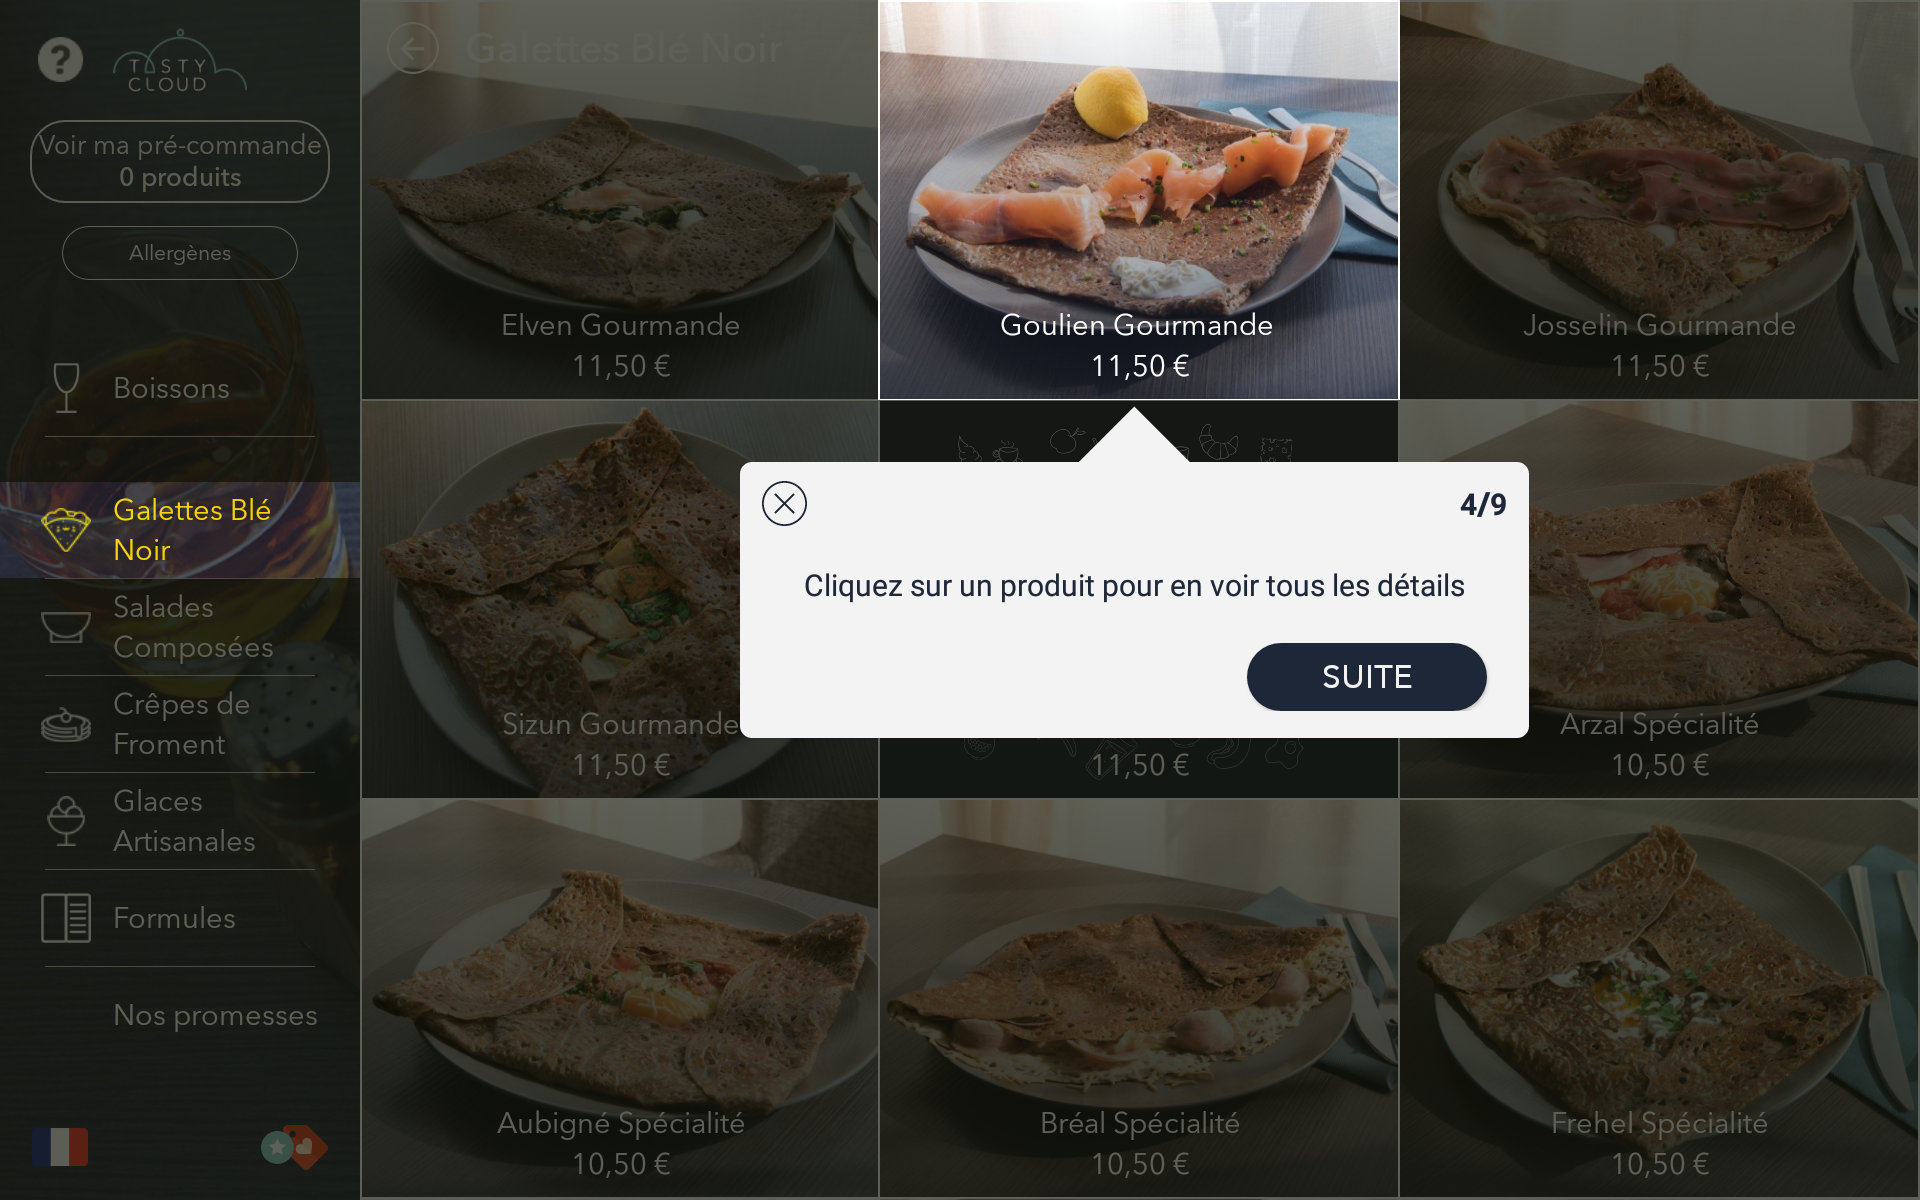
\includegraphics[width=\textwidth]{images/tuto4.png}
    \caption{Étape 4}
  \end{minipage}
\end{figure}

\begin{figure}[!htb]
  \centering
  \begin{minipage}[b]{0.45\textwidth}
    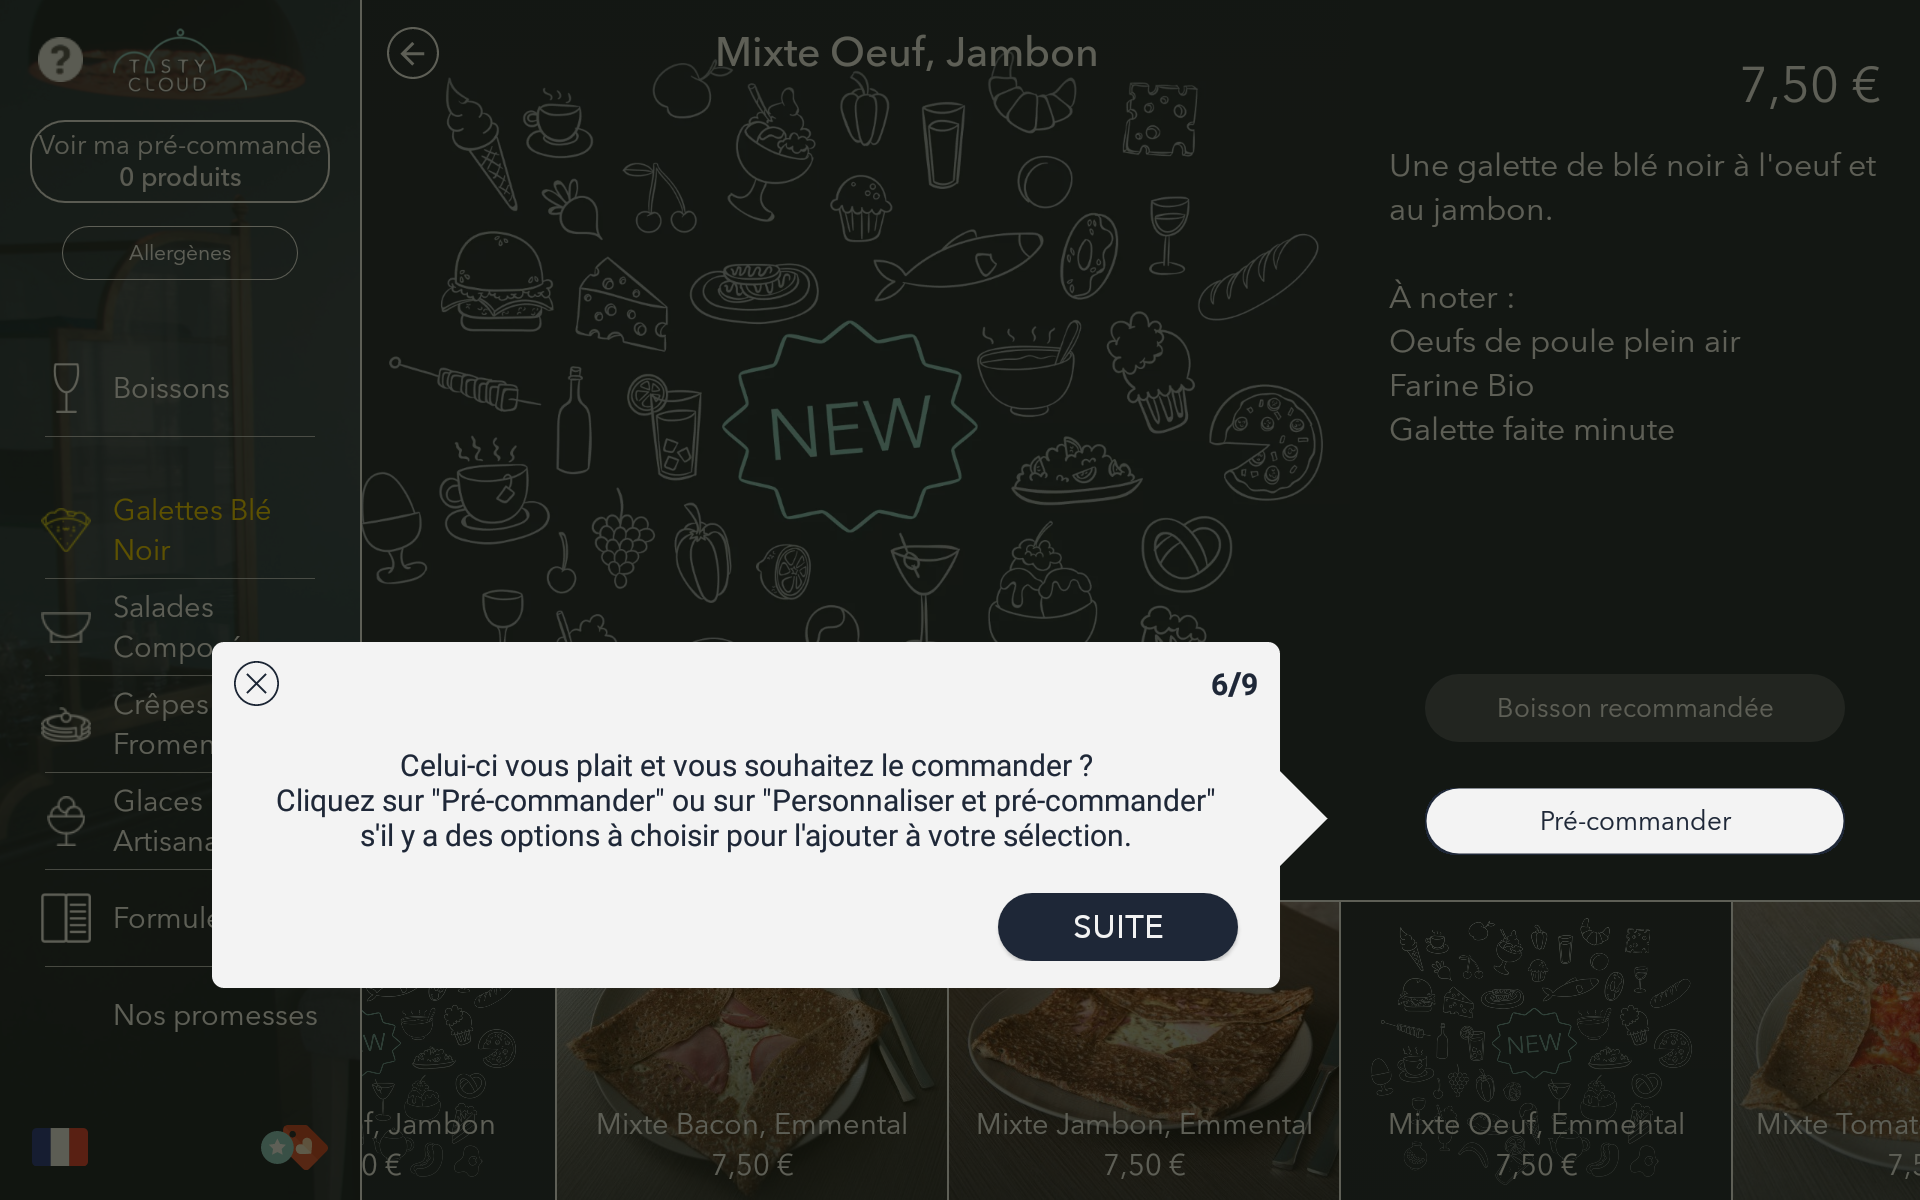
\includegraphics[width=\textwidth]{images/tuto5.png}
    \caption{Étape 6}
  \end{minipage}
  \hfill
  \begin{minipage}[b]{0.45\textwidth}
    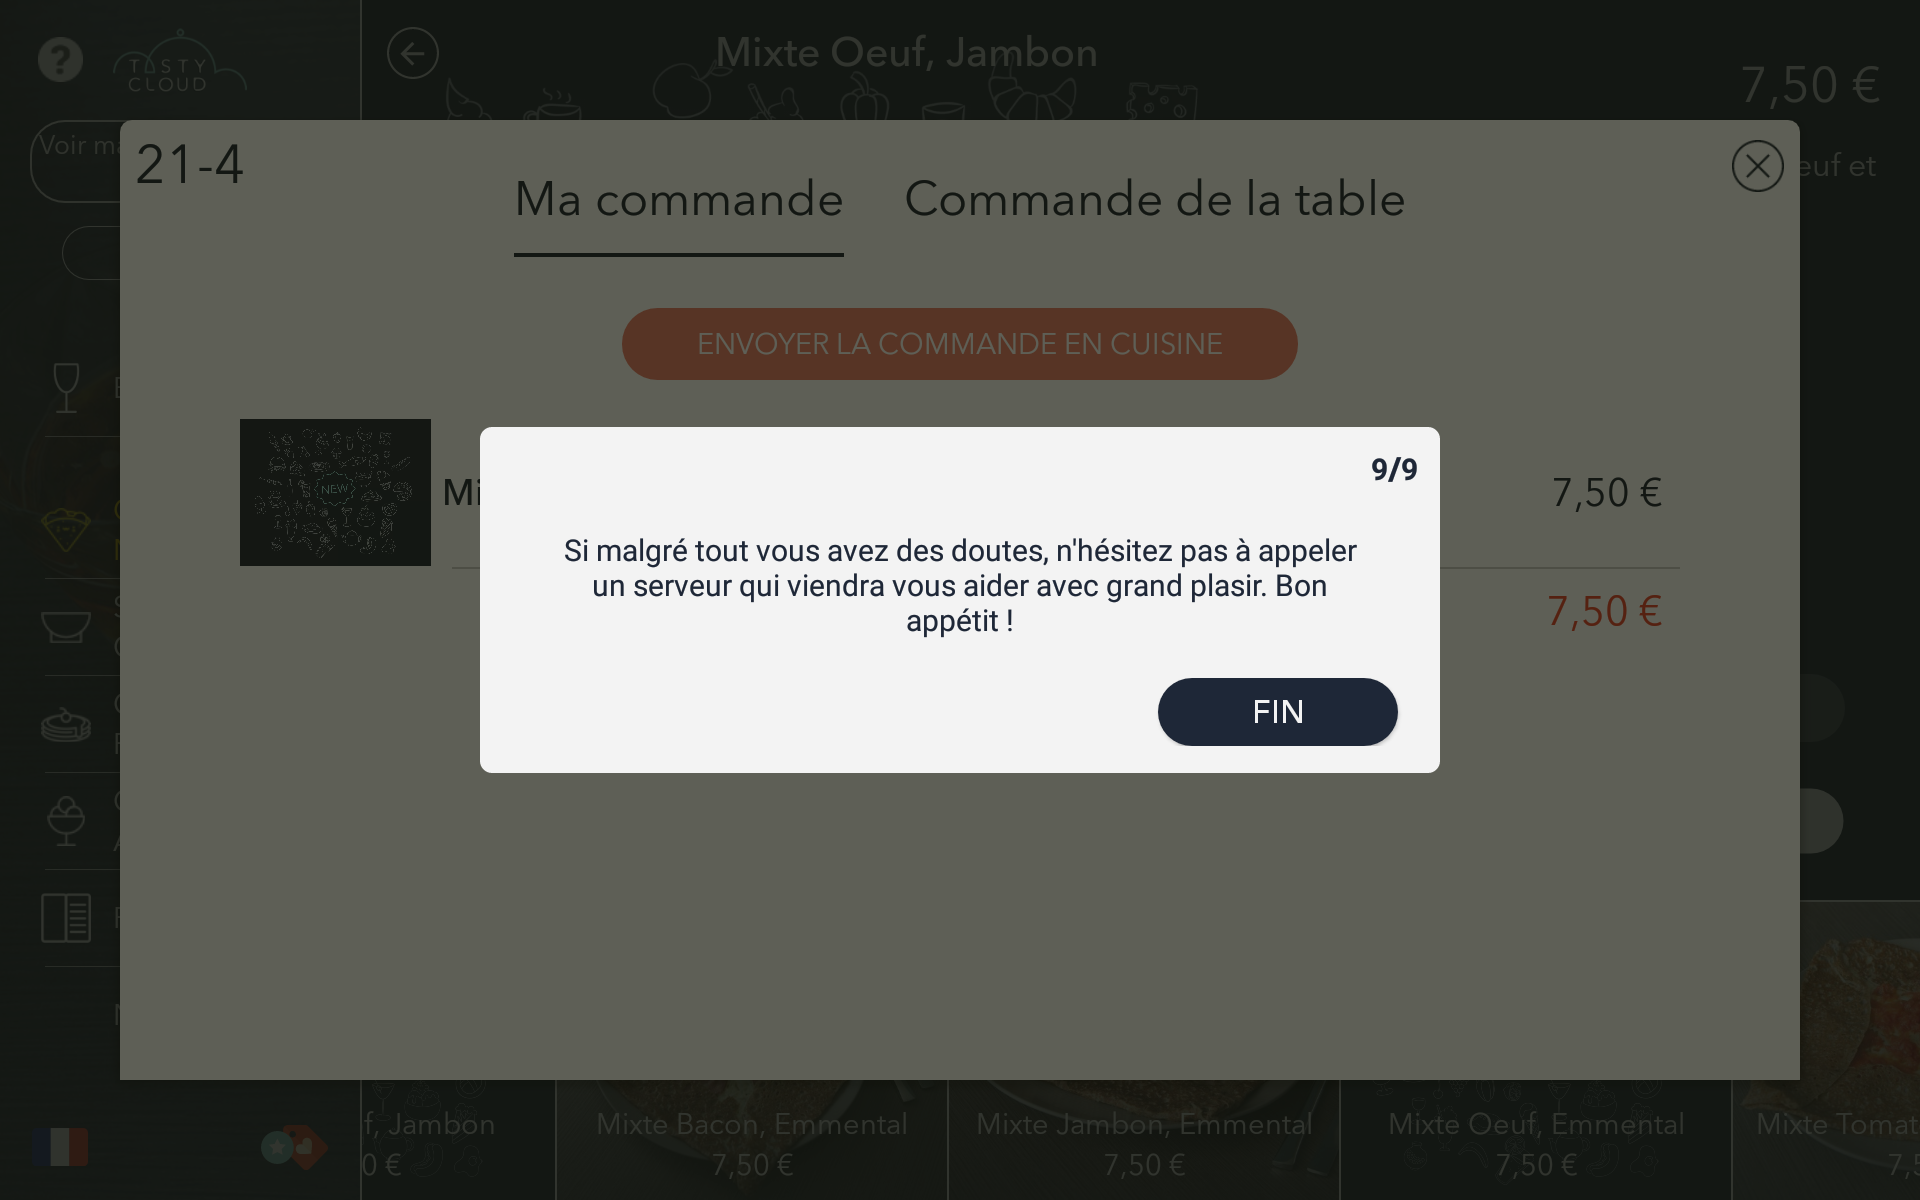
\includegraphics[width=\textwidth]{images/tuto6.png}
    \caption{Étape 9}
  \end{minipage}
\end{figure}

\clearpage

\underline{Code du TouchDelegate}

\begin{lstlisting}[frame=single]  % Start your code-block
    
        fun setExtraRectangleClickable (minView: View, extraTop: Int, 
        extraLeft: Int, extraBottom: Int, extraRight: Int) {

        //initialisation du pere de la vue
        var bigView = minView.parent as View

        bigView.post({
            //recuperation du rectangle entourant la vue
            var rect = Rect()
            minView.getHitRect(rect)

            //ajout des dimensions elargies
            rect.top -= extraTop.dp
            rect.left -= extraLeft.dp
            rect.bottom += extraBottom.dp
            rect.right += extraRight.dp

            //creation du touch delegate
            var touchDelegate = TouchDelegate(rect, minView)
            this.addDelegate(touchDelegate)

            //affectation du delegate au pere
            bigView.touchDelegate = this

        })

    }
    
\end{lstlisting}

\underline{Code du ScrollView :}

\begin{lstlisting}[frame=single]  % Start your code-block
    
   override fun getTopFadingEdgeStrength(): Float {
        if (childCount == 0) {
            return 0.0f
        }

        val length = verticalFadingEdgeLength
        if (scrollY < length) {
            if((scrollY / length.toFloat()) >= 0.2f)
                return 0.2f
            else
                return scrollY / length.toFloat()
        }

        return 0.2f

    }

\end{lstlisting}

On force à toujours retourner 0.2f après un cap

\clearpage
\underline{Page web changées :}

http://www.tastycloud.fr/clients-menu-sur-tablette-tactile.html

http://www.tastycloud.fr/press-restaurant-connecte-digital.html

\chapter{Bibliographie}
\label{sec:bibliographie}

Site web de Tastycloud : 

http://www.tastycloud.fr

Recherche web principalement sur : 

https://stackoverflow.com/

https://developer.android.com/

Aide Kotlin : 

http://tutos-android-france.com/introduction-a-kotlin/




%%% Local Variables: 
%%% mode: latex
%%% TeX-master: "isae-report-template"
%%% End: 






